\chapter{CHAPTER 2 TITLE}
\label{chap:chapter_2}

Hooray for Chapter 2!!!

Sample Figures and Tables below.

And as an example of citing things, here is the \TeX book by Knuth in 1986~\cite{knuth1986texbook}. 

See \verb|bibliography.bib| for doing references.

\begin{figure*}[h]
	\centering
	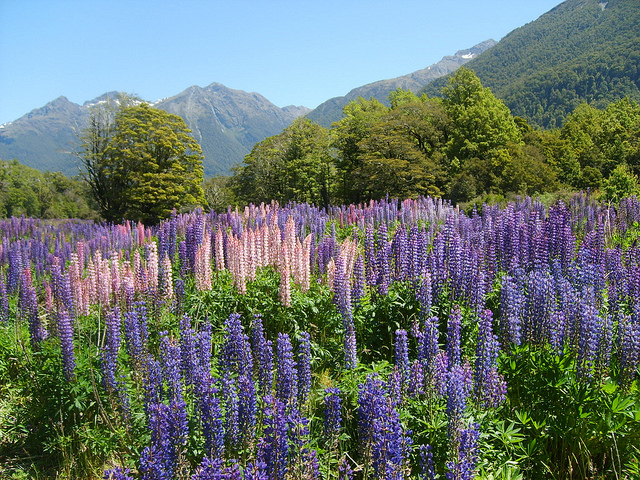
\includegraphics[width=0.7\textwidth]{./Plots/nature.jpg}
	\caption{An individual figure!}
\end{figure*}
        
\begin{figure*}[ht]
	\centering
	\subfloat[\label{fig:HD8538_ellplot}]{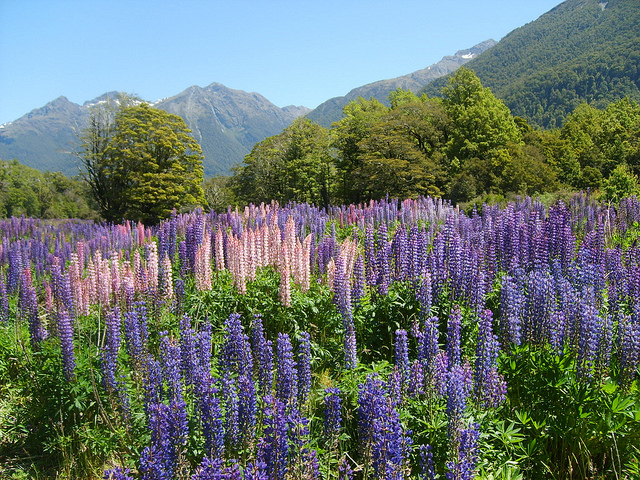
\includegraphics[width=.4\textwidth]{./Plots/nature.jpg}} 
	\subfloat[\label{fig:HD8538_phot}]{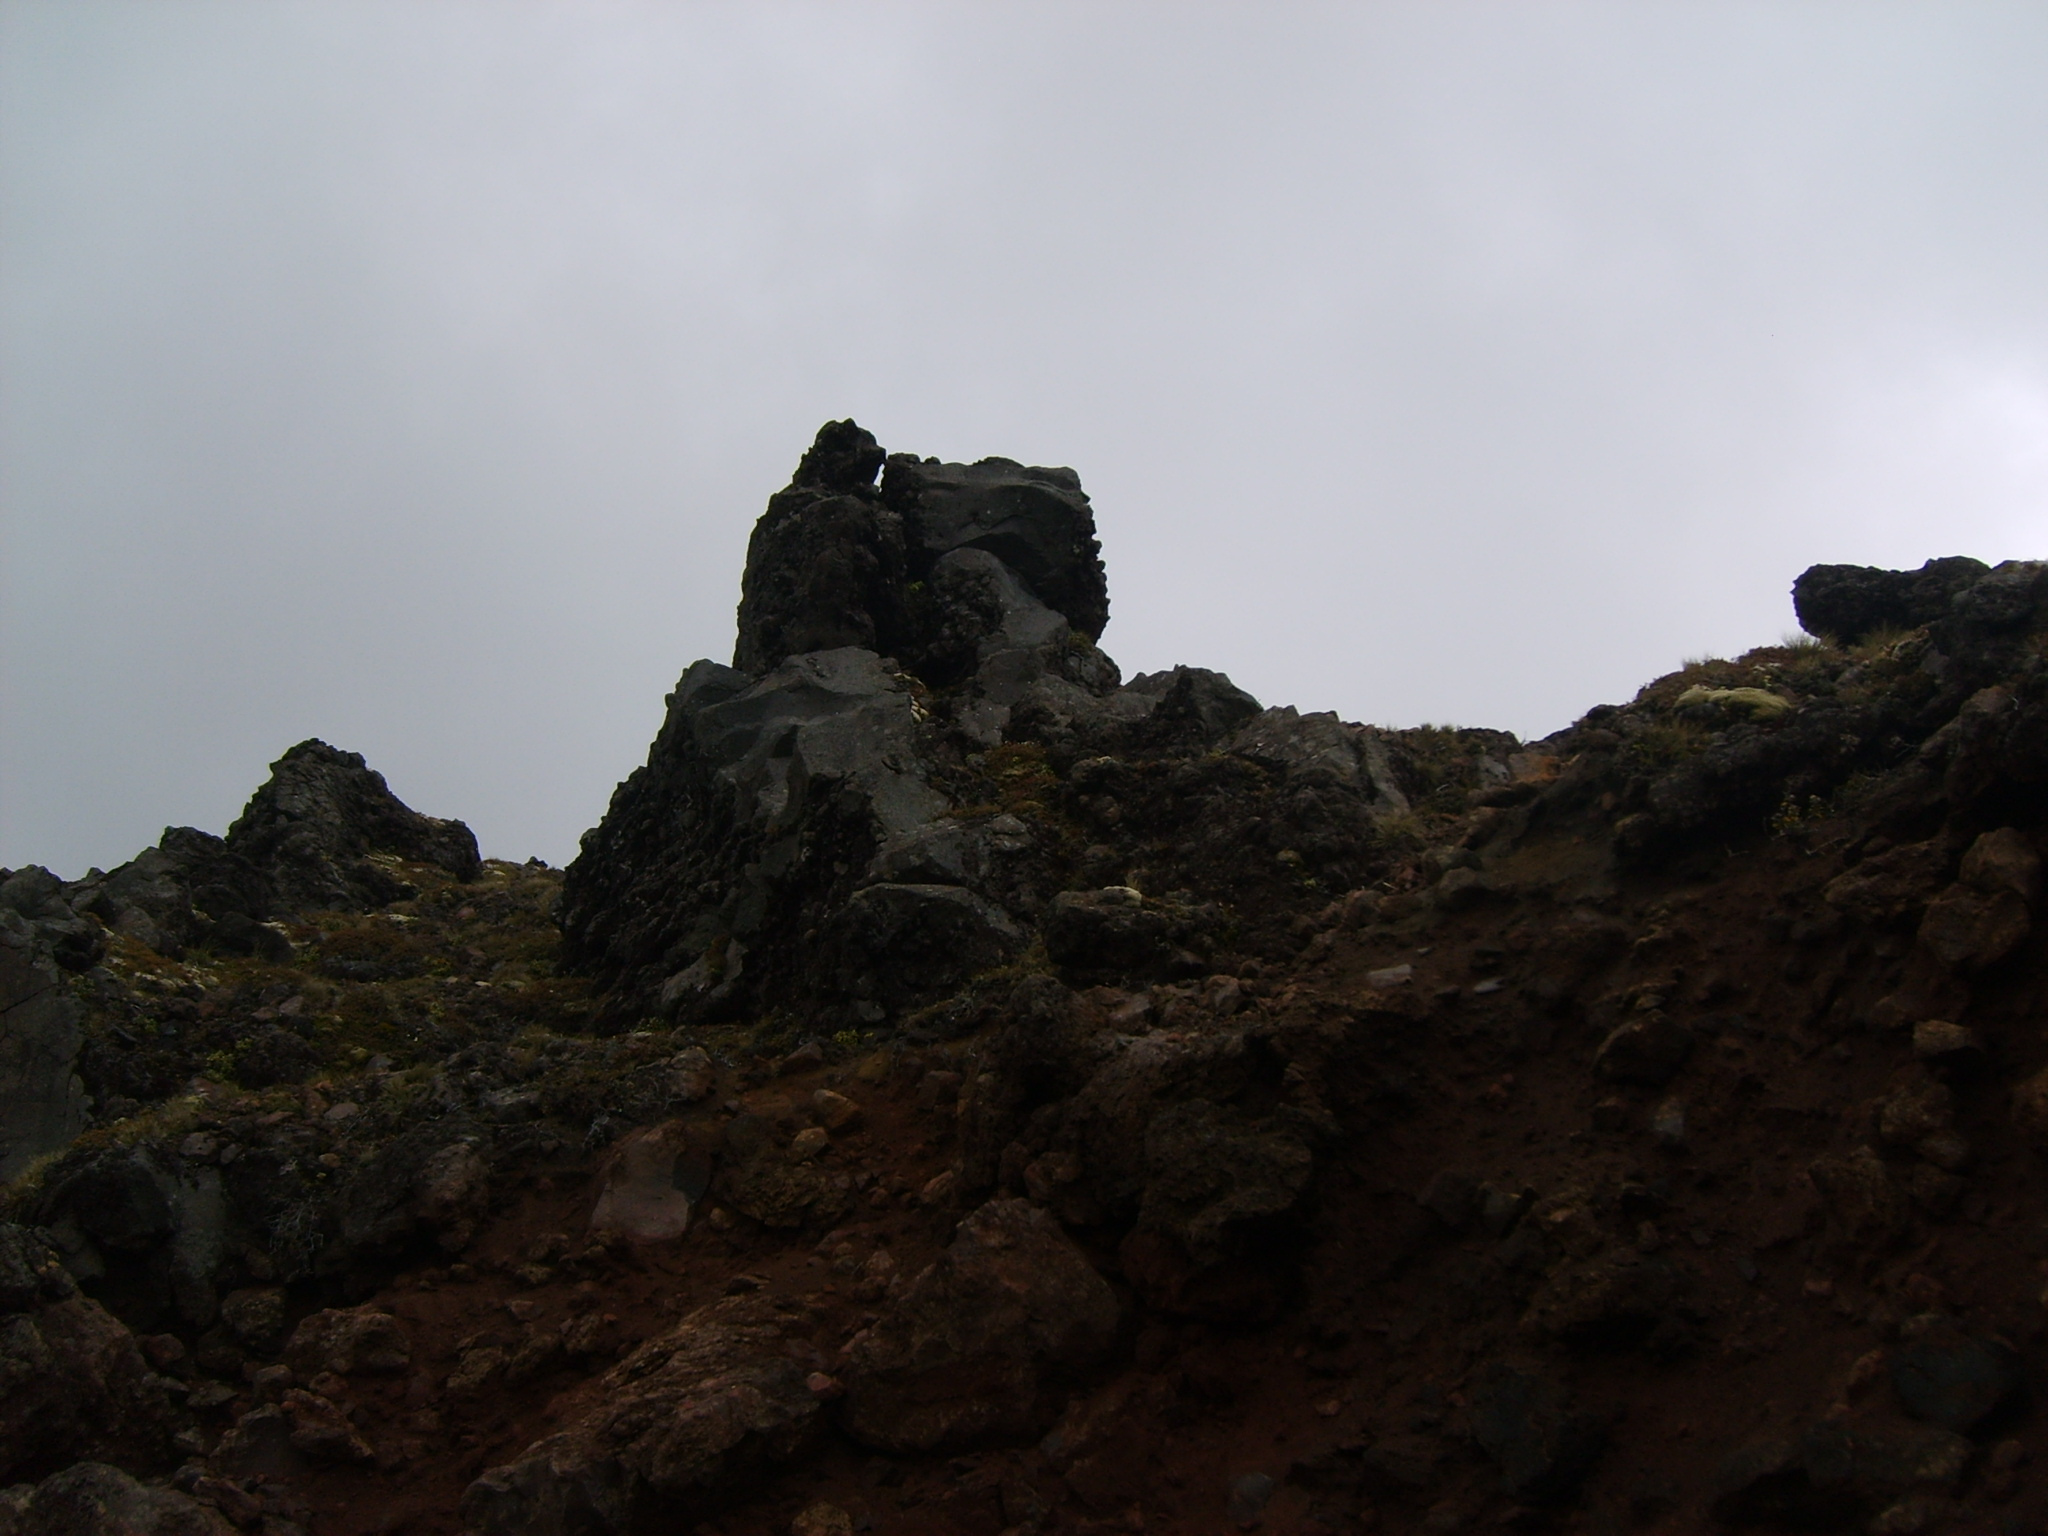
\includegraphics[width=.4\textwidth]{./Plots/rocks.jpg}} \\
	\subfloat[\label{fig:HD8538_vis}]{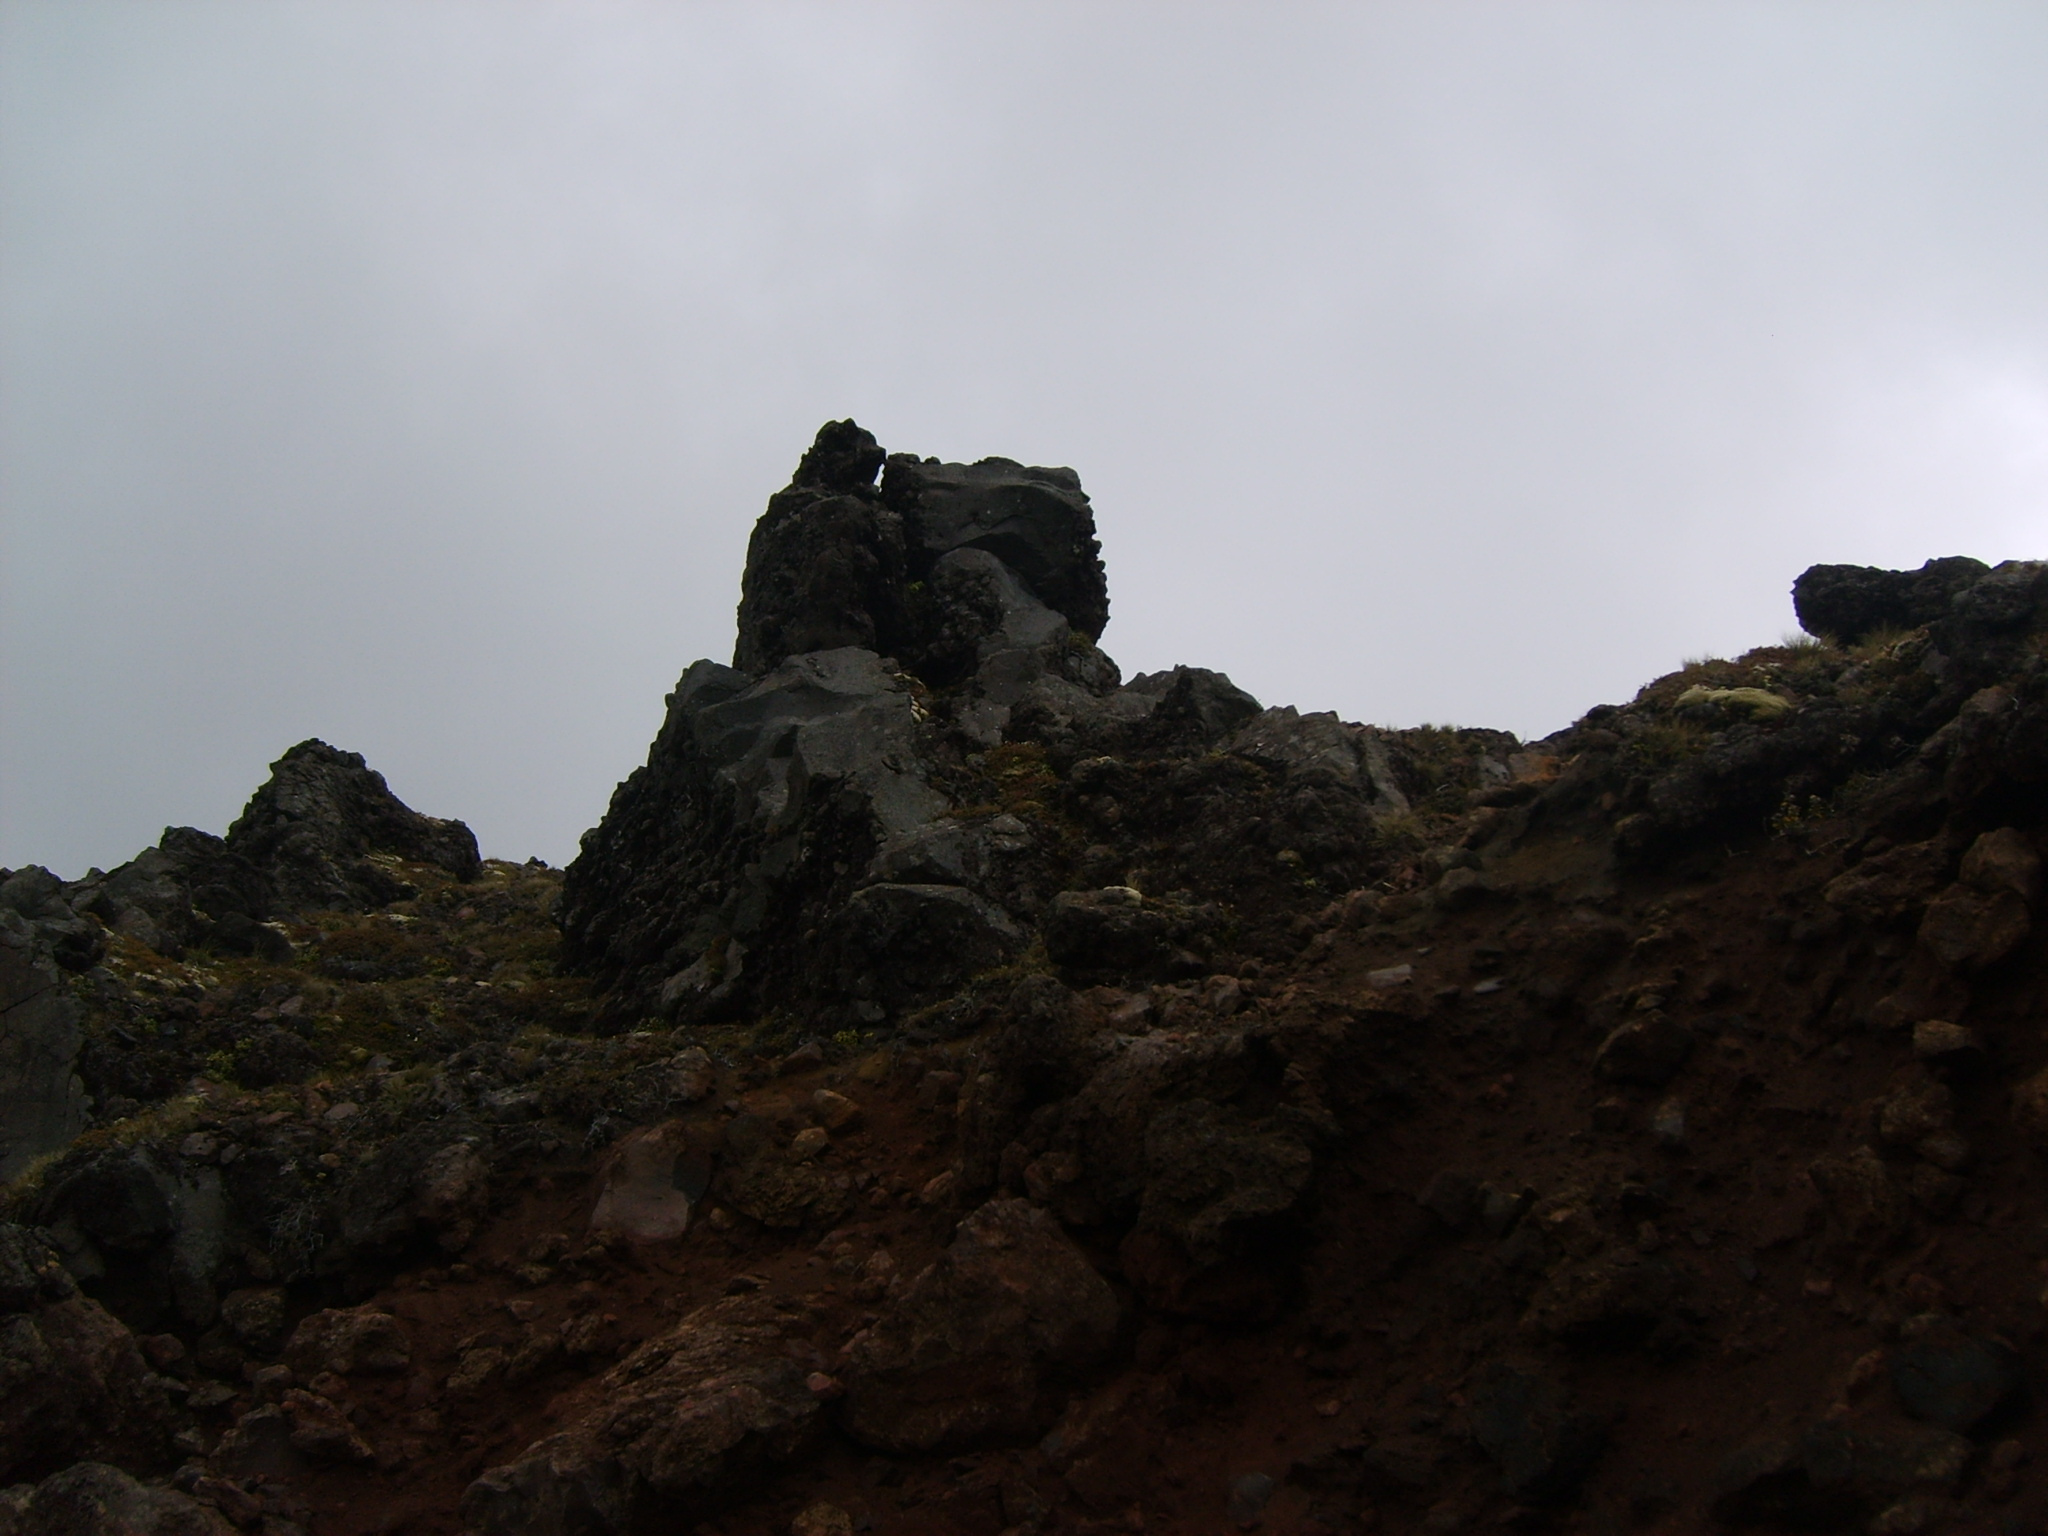
\includegraphics[width=.4\textwidth]{./Plots/rocks.jpg}}
	\subfloat[\label{fig:HD8538_HRD}]{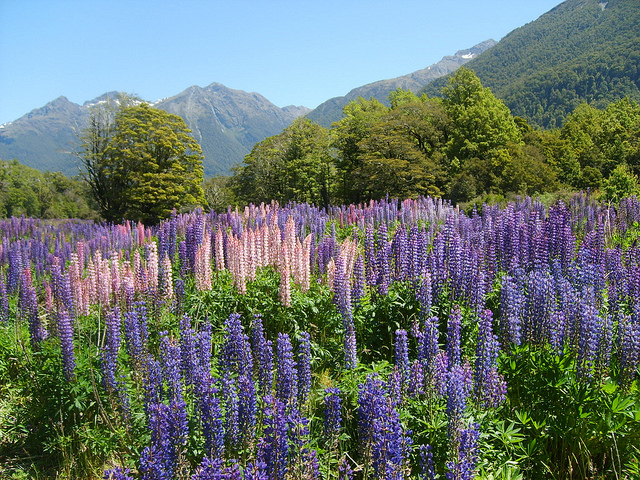
\includegraphics[width=.4\textwidth]{./Plots/nature.jpg}}
	\caption{Multiple figures!}
\end{figure*}

You can have a table like this:
\begin{table}[h!]
	\centering
	\label{tab:simple_table}
	\caption{A simple table}
	\begin{tabular}{|c|c|c|}
		\hline
		\textbf{ID} & \textbf{Name} & \textbf{Course} \\
		\hline
		1 & John Doe & Mathematics \\
		2 & Jane Smith & Physics \\
		3 & Mary Johnson & Chemistry \\
		\hline
	\end{tabular}
\end{table}

You can also include a wide table like this:

\begin{landscape}
\begin{longtable}{cccccccccccccc}
\label{tab:wide_table_example}\\
\caption{An example of very large horizontal table}\\
\hline\endhead  % header material
\hline\endfoot  % footer material
\hline
\textbf{ID} & \textbf{Name} & \textbf{Age} & \textbf{Email} & \textbf{Phone} & \textbf{Major} & \textbf{Grade} & \textbf{Comments} \\
\hline
1 & John Doe & 20 & johndoe@example.com & 123-456-7890 & Mathematics & A & Excellent work \\

2 & Jane Smith & 22 & janesmith@example.com & 234-567-8901 & Physics & B & Good understanding \\

3 & Mary Johnson & 21 & maryjohnson@example.com & 345-678-9012 & Chemistry & A & Outstanding performance \\

4 & James Brown & 23 & jamesbrown@example.com & 456-789-0123 & Biology & C & Needs improvement \\

5 & Patricia Davis & 20 & patriciadavis@example.com & 567-890-1234 & English & B & Well done \\

6 & Robert Miller & 22 & robertmiller@example.com & 678-901-2345 & History & A & Excellent analysis \\

7 & Jennifer Wilson & 21 & jenniferwilson@example.com & 789-012-3456 & Geography & B & Good research \\

8 & Michael Moore & 23 & michaelmoore@example.com & 890-123-4567 & Computer Science & A & Great coding skills \\

9 & Linda Taylor & 20 & lindataylor@example.com & 901-234-5678 & Art & C & More practice needed \\

10 & William Anderson & 22 & williamanderson@example.com & 012-345-6789 & Music & B & Good performance \\
\hline
\end{longtable}
\end{landscape}
